\chapter{Lower IR and Control Flow}
\label{chap:lower-ir}

After semantic analysis and compile-time evaluation, the compiler lowers
\irtree{} into a lower intermediate representation. This lower IR is closer to
machine code and LLVM. It is built around functions, basic blocks, instructions,
terminators, values, definitions, and allocation slots. This chapter explains
the representation and the lowering process.

\section{Purpose of Lower IR}

\irtree{} is convenient for semantic analysis because it keeps expression
structure. LLVM generation, however, needs explicit control flow. It must know
which basic block branches to which successor, where values merge, where returns
happen, and which operations produce reusable values. Lower IR provides this
explicit structure.

The lower IR is not intended to be a full optimizer's IR. It does not implement
dominance analysis, liveness analysis, register allocation, or source-variable
SSA conversion. It is a pragmatic bridge between typed \irtree{} and LLVM IR.
It makes enough structure explicit that LLVM generation can be systematic.

\section{Functions and Basic Blocks}

An IR function contains a mangled name, argument types, a variadic flag, a return
type, and optionally a body. A body contains a list of allocation slots, an entry
basic block ID, and a map of basic block IDs to blocks. A basic block contains
block arguments, instructions, and a terminator.

Block arguments are important. When a conditional or loop produces a value, the
continuation block receives that value as a block argument. During LLVM
generation, block arguments become phi nodes. This avoids carrying explicit phi
instructions in lower IR while still modeling value merging.
Figure~\ref{fig:block-args} illustrates the four-block pattern produced by a
conditional that yields a value.

\begin{figure}[H]
  \centering
  \fbox{\begin{minipage}{0.88\textwidth}
  \centering
  \begin{tabular}{ccc}
  entry block & $\rightarrow$ & condition block \\
              &               & $\swarrow \quad \searrow$ \\
              &               & true block \quad false block \\
              &               & $\searrow \quad \swarrow$ \\
              & $\leftarrow$  & continuation block with block argument
  \end{tabular}
  \end{minipage}}
  \caption{Value merge represented by a continuation block argument}
  \label{fig:block-args}
\end{figure}

\section{Values and Definitions}

Lower IR values can be zero-sized values, undefined values, booleans, strings,
numbers, or definitions. A \texttt{DefinitionId} represents the result of an
instruction or a block argument. Each definition has a type.

This gives the IR an SSA-like property for computed values: an instruction
produces a fresh definition, and later instructions refer to it. Source
variables are different. Mutable locals are represented as allocation slots, so
assignments become stores and reads become loads. This hybrid design is simple
and maps naturally to LLVM \texttt{alloca}, \texttt{load}, and \texttt{store}.

\section{Instructions}

The lower IR instruction set is small:

\begin{itemize}
  \item \texttt{Load} reads from a pointer value.
  \item \texttt{Store} writes a value to a pointer value.
  \item \texttt{FunctionCall} calls a named function.
  \item \texttt{Cmp} compares integer or boolean values.
  \item \texttt{Arithmetic} performs integer arithmetic.
  \item \texttt{Not} negates a boolean.
  \item \texttt{OffsetPtr} computes a byte offset from a pointer.
  \item \texttt{Zext}, \texttt{Sext}, and \texttt{Truncate} implement integer
        casts.
\end{itemize}

Terminator instructions are separate from ordinary instructions. A block ends in
a jump, conditional jump, return, or unreachable terminator. This separation
prevents accidentally appending instructions after control flow has already left
the block.

\section{Type Lowering}

The lower IR type system is simpler than the \irtree{} type system. The
\irtree{} distinguishes signed and unsigned integers. Lower IR collapses
\texttt{i8}/\texttt{u8} into \texttt{I8}, \texttt{i32}/\texttt{u32} into
\texttt{I32}, and \texttt{i64}/\texttt{u64} into \texttt{I64}. Signedness is not
stored in the type. Instead, the lowering stage attaches a \texttt{signed}
boolean to arithmetic, comparison, and extension instructions where signedness
matters.

Pointers become a single lower \texttt{Ptr} type. Structs become lower struct
types with field types and layout. Arrays become lower array types. The never
type is lowered to unit because a never expression does not produce a normal
value in lower IR.

\section{Lowering Blocks and Locals}

When lowering a \irtree{} block, the compiler creates an allocation slot for
each variable declared in the block. It stores the mapping from \texttt{VariableId}
to allocation definition in \texttt{variable\_map}. Then it evaluates the block's
expressions in order. If an expression returns \texttt{Never}, the block returns
\texttt{Never} to its caller, because following expressions are unreachable.

This model is simple but not fully optimized. Every local variable becomes a
stack slot even if it could be represented as an SSA value. LLVM can later
optimize many such allocas in production optimization pipelines, but this
compiler currently emits unoptimized object code. The choice is appropriate for
the project because it keeps assignment, address-of, field updates, and array
updates uniform.

\section{Lowering Places}

Places lower to pointers. A variable place lowers to the allocation slot for
that variable. A dereference place lowers by evaluating the pointer expression.
A field place lowers by computing the field offset and emitting an
\texttt{OffsetPtr}. An array element place lowers by evaluating the array pointer
and index, multiplying the index by the element size, and emitting
\texttt{OffsetPtr}.

This is one of the reasons the place/value distinction in \irtree{} is useful.
By the time lower IR generation runs, it can ask for a place as a pointer and
generate load or store instructions around it.

\section{Lowering Conditionals}

When lowering an \texttt{If} expression, the compiler creates three blocks: the
true block, the false block, and the continuation block. It evaluates the
condition in the current block and emits a conditional jump to the true and false
blocks. Each branch is then lowered independently. If a branch produces a value,
it jumps to the continuation block and passes the value as an argument. If a
branch never returns, it does not jump to the continuation. The continuation
block receives a fresh block argument representing the value of the whole
\texttt{If} expression.

This works for both ordinary conditionals and lowered short-circuit boolean
operators. Because \texttt{a || b} has already become an \texttt{If}, lower IR
does not need a separate short-circuit instruction.

\section{Lowering Loops}

Loop lowering creates a body block and a continuation block. The current block
jumps to the body block. \texttt{continue} jumps to the body block. \texttt{break}
jumps to the continuation block and passes the break value as an argument. If
the loop body reaches the end normally, the compiler emits a jump back to the
body block.

The lowering context stores maps from \texttt{LoopId} to break and continue
targets. This is why \texttt{LoopId} is assigned during \irtree{} lowering.
Nested loops work because each \texttt{break} and \texttt{continue} carries the
specific loop ID it targets.

\section{Aggregates}

Struct and array values require special handling. A simple scalar expression can
be evaluated to a lower IR value directly. An aggregate initializer may require
writing several fields or elements into memory. The lowering context therefore
has helper methods that evaluate array initializers and struct initializers into
a provided pointer.

For a struct initializer, the compiler evaluates field expressions, computes
each field offset from the semantic type layout, and stores each value into the
appropriate offset. For an array initializer, it evaluates all element
expressions, computes each element offset from the element layout, and stores
the values in order. Constants for aggregate values are lowered similarly by
allocating storage, writing the constant into that storage, and loading the
aggregate value.

\section{Cleanup Passes}

After lowering, \texttt{ir::opt::basic\_passes} runs two passes:
\texttt{drop\_zst} and \texttt{simplify\_cfg}.

\texttt{drop\_zst} removes operations on zero-sized types. It removes zero-sized
function arguments, block arguments, allocation slots, loads, stores, and
normalizes zero-sized returns. This matters because \texttt{unit} is represented
as a type in the compiler but should not create useless run-time memory
operations.

\texttt{simplify\_cfg} removes unreachable blocks, merges a block with its only
successor when the successor has a single predecessor, and redirects empty jump
blocks to their targets. It also maintains a rename map so references to merged
block arguments are updated correctly.

These passes are small, but they improve the readability of lower IR and make
LLVM generation simpler. They also demonstrate how compiler optimizations can
start with local transformations before moving to more advanced analyses.

\section{Graphviz Output}

The \texttt{cfg} command renders lower IR as a Graphviz DOT graph. Each function
becomes a subgraph. Each basic block is shown with its arguments, instructions,
and terminator information. Edges show jumps and conditional branches. This is a
debugging feature, but it is also useful for learning. Many compiler concepts
are easier to understand when control flow is visible as a graph instead of only
as a linear debug dump.

The following two examples illustrate how source language constructs map to
basic blocks in the generated CFG.

Listing~\ref{lst:select-src} shows a function that selects between two values
using a conditional expression. The generated CFG in
Figure~\ref{fig:cfg-select} reveals the four-block structure produced by
conditional lowering: an entry block that evaluates \texttt{flag} and emits a
conditional jump, a true block, a false block, and a continuation block that
receives the selected value as a block argument.

\begin{lstlisting}[language=EPL,caption={select.epl: conditional expression},label={lst:select-src}]
fn select(a: i32, b: i32, flag: bool) -> i32 {
    if flag { a } else { b }
}
\end{lstlisting}

\begin{figure}[H]
  \centering
  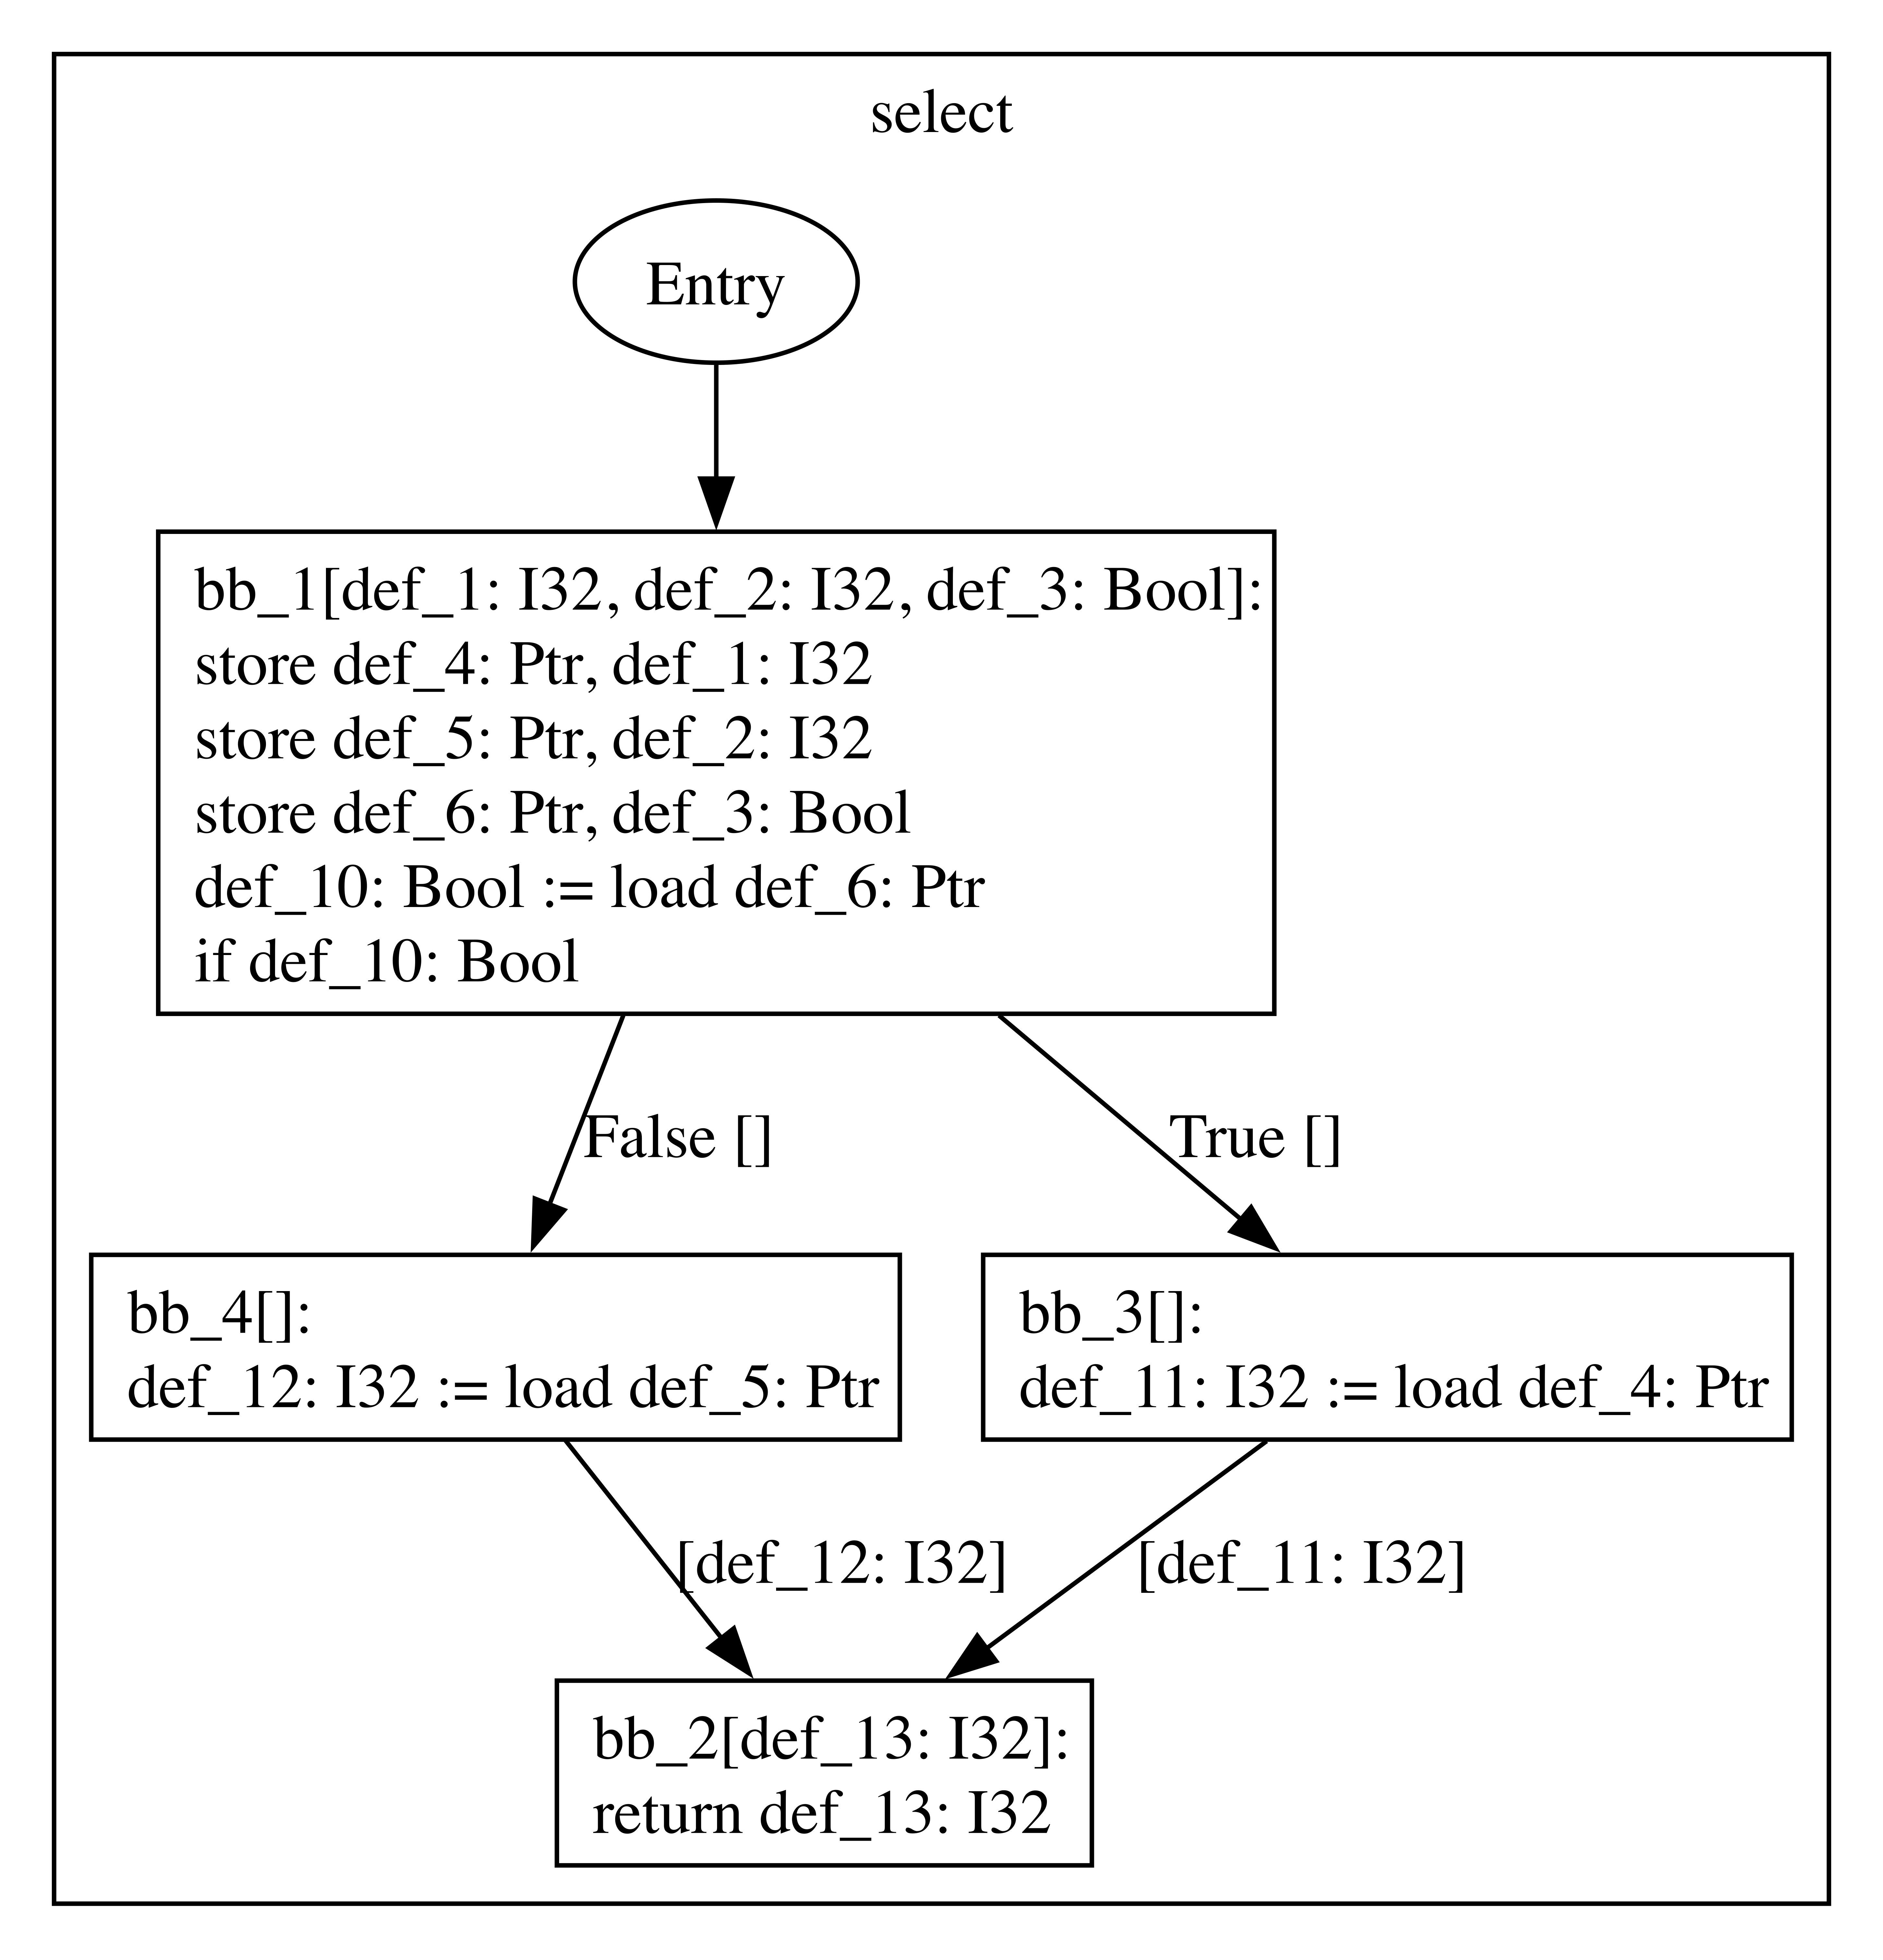
\includegraphics[width=0.9\textwidth]{images/select.png}
  \caption{CFG for \texttt{select}: entry block branches to the true and false
           blocks, which both pass their result to a shared continuation block
           argument}
  \label{fig:cfg-select}
\end{figure}

Listing~\ref{lst:sum-range-src} shows a function that accumulates a sum over a
range using a \texttt{while} loop. The generated CFG in
Figure~\ref{fig:cfg-sum-range} shows the loop structure: an entry block that
falls through to the body block, a body block that performs the loop work and
loops back to itself via a conditional jump, and a continuation block reached
when the loop condition is false.

\begin{lstlisting}[language=EPL,caption={sum\_range.epl: while loop accumulation},label={lst:sum-range-src}]
fn sum_range(from: i32, to: i32) -> i32 {
    let sum = 0;
    while from < to {
        sum += from;
        from += 1;
    }
    sum
}
\end{lstlisting}

\begin{figure}[H]
  \centering
  \includegraphics[width=0.9\textwidth]{images/sum_range.png}
  \caption{CFG for \texttt{sum\_range}: the body block loops back to itself
           while the condition holds, and exits to the continuation block when
           the condition fails}
  \label{fig:cfg-sum-range}
\end{figure}

\section{Tradeoffs}

The lower IR is intentionally pragmatic. It is not a research-grade SSA
optimizer. It does not eliminate all loads and stores, it does not perform
constant propagation, it does not inline functions, and it does not select
machine instructions. Instead, it provides exactly the structure needed to
bridge \irtree{} and LLVM.

This is the right tradeoff for \epl{} because LLVM already provides a strong
backend. The project value is in showing the full path from source language
design to LLVM generation, not in replacing LLVM's optimizer or target
infrastructure.
